%!TEX root=../mythesis.tex
% Chapter Template

\chapter{Shared Encoders} % Main chapter title
\chaptermark{Shared Encoders}  % replace the chapter name with its abbreviated form
\label{ch:shared_encoders}


\section{Method}\label{sec:shared_encoders_methods}


\begin{figure}[!htbp]
	\centering
	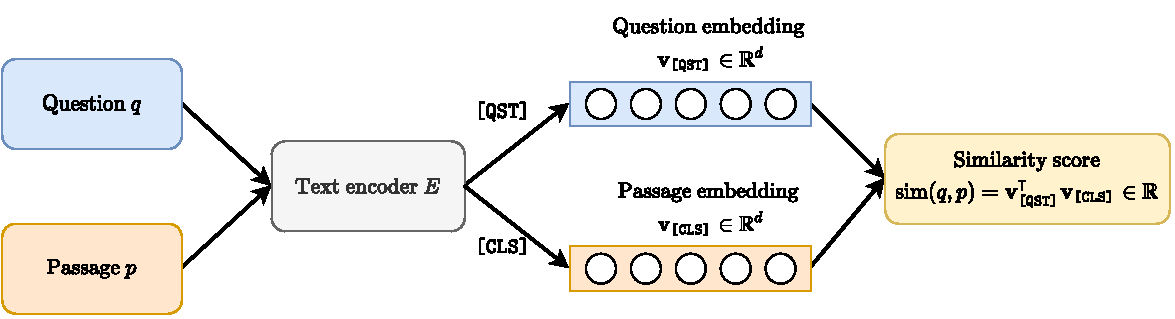
\includegraphics[width=0.9\linewidth]{shared_encoders/two_tower_shared.pdf}
	\caption[Two-tower architecture of DPR retriever with parameter sharing.]{
		%
		The two-tower architecture of the DPR retriever with parameter sharing.
		%
		The same encoder will encode input texts into their embedding vectors with proper special tokens \texttt{[QST]} or \texttt{[CLS]} to distinguish the input types.
	}
	\label{fig:two_tower_shared}
\end{figure}


%
In this chapter, we present our first contribution to the DPR architecture~\cite{karpukhin2020dense} -~\emph{shared encoders}.
%
Recall that the two-tower DPR retriever consists of a question encoder $E_Q$ and a passage encoder $E_P$ with the same architecture (i.e., BERT~\cite{devlin2019bert}) but different weights~\footnote{In the context of deep learning,~\emph{weights} refers to the values of the parameters of the model.}.
%
In this setup, the task of both encoders is to textual data to the same embedding space, one being question texts and one being passage texts.
%
Therefore, it emerges naturally that sharing parameters of these two models could be beneficial.

%
More specifically, we use the same set of parameters for the two encoders while assigning the special token \texttt{[CLS]} to the passage encoder and \texttt{[QST]} to the question encoder.
%
The similarity score between a question $q$ and a passage $p$ defined in~\eqref{eq:sim_score} then becomes:
%
\begin{equation}
\text{sim}(q, p) = \mathbf{v}^\intercal_{\texttt{[QST]}} \mathbf{v}_{\texttt{[CLS]}} \in \mathbb{R}
\end{equation}
%
~\fref{fig:two_tower_shared} illustrates the architectural design of this approach.
%
Under this architecture, we allow the models to share the general world knowledge and natural language understanding capabilities and at the same time to distinguish the input types.
%
Furthermore, this approach can be seen as a multi-task training algorithm, in which the general encoder $E$ is trained to map both questions and passages to the same feature space.


\section{Experimental Results}\label{sec:shared_encoders_results}


\begin{table*}[t!]
	\setlength\tabcolsep{5pt}
	\centering
	\small
	\begin{tabular}{ll|cccc}
		\toprule
		\textbf{Negative type} & \textbf{Retriever}
		& Top-1 & Top-5 & Top-20 & Top-100 \\ 
		\midrule
		\multirow{2}{*}{BM25} & DPR & 42.01 & 64.54 & 76.48 & 84.29 \\
		&DPR (shared encoders) & \textbf{45.01} & \textbf{66.70} & \textbf{78.25} & \textbf{85.62} \\
		\midrule
		\multirow{2}{*}{DPR hard negatives} & DPR & 49.36 & 67.34 & 78.09 & 85.40 \\
		& DPR (shared encoders) & \textbf{53.02} & \textbf{71.30} & \textbf{80.89} & \textbf{86.93} \\
		\bottomrule
	\end{tabular}
	\caption[Top-$\{1, 5, 20, 100\}$ retrieval accuracy on the Natural Questions test set of the DPR retriever with and without parameter sharing.]{
		%
		Top-$\{1, 5, 20, 100\}$ retrieval accuracy on the Natural Questions test set, calculated as the percentage of top-$k$ retrieved passages that contain the answer.
		%
		We present the results on training with two different negative types, BM25 or hard negatives.
		%
		The proposed shared encoders approach consistently and substantially outperforms the baseline DPR model on various settings with no additional cost.	
}
	
	\label{tab:shared_encoders_results}
\end{table*}


We provide the retrieval results on NQ in~\tref{tab:shared_encoders_results}, where we train the DPR model with BM25 hard negative passages described in~\sref{sec:dpr_training} and DPR hard negative passages, respectively.
%
In the latter case, negative passages are obtained by performing retrieval with a DPR checkpoint then for each question taking the highest-scoring passage that does not contain the answer.
%
We note that our results on the original DPR architecture do not match those reported in the original paper~\cite{karpukhin2020dense}, as we trained all these models with a batch size of 24 instead of 128 given our computation budget.
%
Nevertheless, we observe a consistent and considerable improvement of the shared encoders across different training settings and different top-$k$ evaluation.
%
This attests to our hypothesis earlier that this approach allows knowledge sharing and multi-task training that are beneficial to the model performance.

%
Intriguingly, we observe that the improvement of the shared encoders over the DPR baseline is consistently higher with DPR hard negatives than BM25 hard negatives.
%
For example, for top-5 retrieval accuracy, the performance gain of DPR shared encoders with DPR hard negatives is 3.96 points which is almost double of that with BM25 hard negatives (2.16 points).
%
This is opposite to the general intuition that it becomes increasingly difficult to improve a model when its performance is increased.
%
We hypothesize that this attributes to the knowledge sharing power of shared encoders, which can capitalize more on such informative negatives as DPR hard negatives.

%
Additionally, we note that by sharing the parameters of the two encoders, we effectively reduce the memory footprint by half.
%
This is especially critical in retrieval training where in-batch negatives are used, hence gradient accumulation is not sufficient to accommodate for a smaller batch size.
%
We expect the shared encoders to outperform the baseline DPR model even further when trained on a larger batch size, which is an advantage of shared encoders brought about by the memory efficiency of the architectural design.
%
We leave it to a future work to empirically verify this hypothesis.

%
Finally, we note that given its efficiency and effectiveness, we treat the DPR retriever with shared encoders as the baseline DPR model for all subsequent experiments, unless otherwise noted.